\section{Comparativo \texorpdfstring{$M$}{M}-QAM vs. \texorpdfstring{$M$}{M}-PSK}


\begin{itemize}
    \item Para o caso do $M$-QAM é possível observar que ao aumentar o número de símbolos na constalação, há o ganho de símbolos transmitidos por símbolos. Ao manter a energia $\mathcal{E}_g$ fixa, a energia média da constelação cresce porporcionalmente. Sendo igual 1, 10 e 21 para os casos de M ={4,16,64}, respectivamente. Isso implicada que a distância $d$ entre os símbolos adjacentes é a mesma, acarretando limiares que exigem atenção do engenheiro. É possível observar na figura~\ref{fig:Erro_teoricaxAWGN_Geral} que para $M = \{16, 64\}$, é necessária a \textit{SNR} $\geq \{12, 20\}$ dB para ter uma taxa de erro de símbolo menor que 0.1.
    \item O item anterior indica que há uma exigência de um sistema de transmissão mais robusto ao ruído, pois aumentando a quantidade de símbolos, há uma maior influência do ruído, de forma a deteriorar totalmente a informação enviada dado a proximidade dos símbolos. A transmissão é totalmente prejudicada e equivale ao experimento de jogar uma moeda para saber se o símbolo recebido está correto ou não, já que chega ao ponto de o receptor errar a taxa de 0.5 dos símbolos enviados no caso 64-QAM para 0dB.
    \item Interessante notar a diferença entre a taxa de erro de bit (\textit{BER}) e a taxa de símbolo (\textit{SER}), pois ao utilizar a codificação de Gray o símbolos decidido apresenta apenas um bit de diferença símbolos vizinhos, garantindo que mesmo ao decodificar um símbolo equivocado, a mensagem será afetada de apenas um bit.
    \item Vale notar que há uma diferença entre a energia média ($\mathcal{E}_{media}$) das constelações $M$-QAM e $M$PSK para $M=4$, sendo que estas são identicas, entretanto a segunda apresenta uma ($\mathcal{E}_{media}$) duas vezes menor que a primeira.
    \item As figuras~\ref{fig:Erro_teoricaxAWGN_Geral} e \ref{fig:BER_teoricaxAWGN_Geral} indicam que há uma melhor eficiência espectral para constelações menores, pois estas necessitam de menos energia para alcançar taxas de erros desprezíveis. Entretanto, isto vem com a limitação do número de bits enviados por símbolo e o desafiador é encontrar a relação ideal entre eficiência espectral e bits/símbolo para garantir o o melhor resultado.
\end{itemize}

\begin{figure}[!ht]
    \centering
    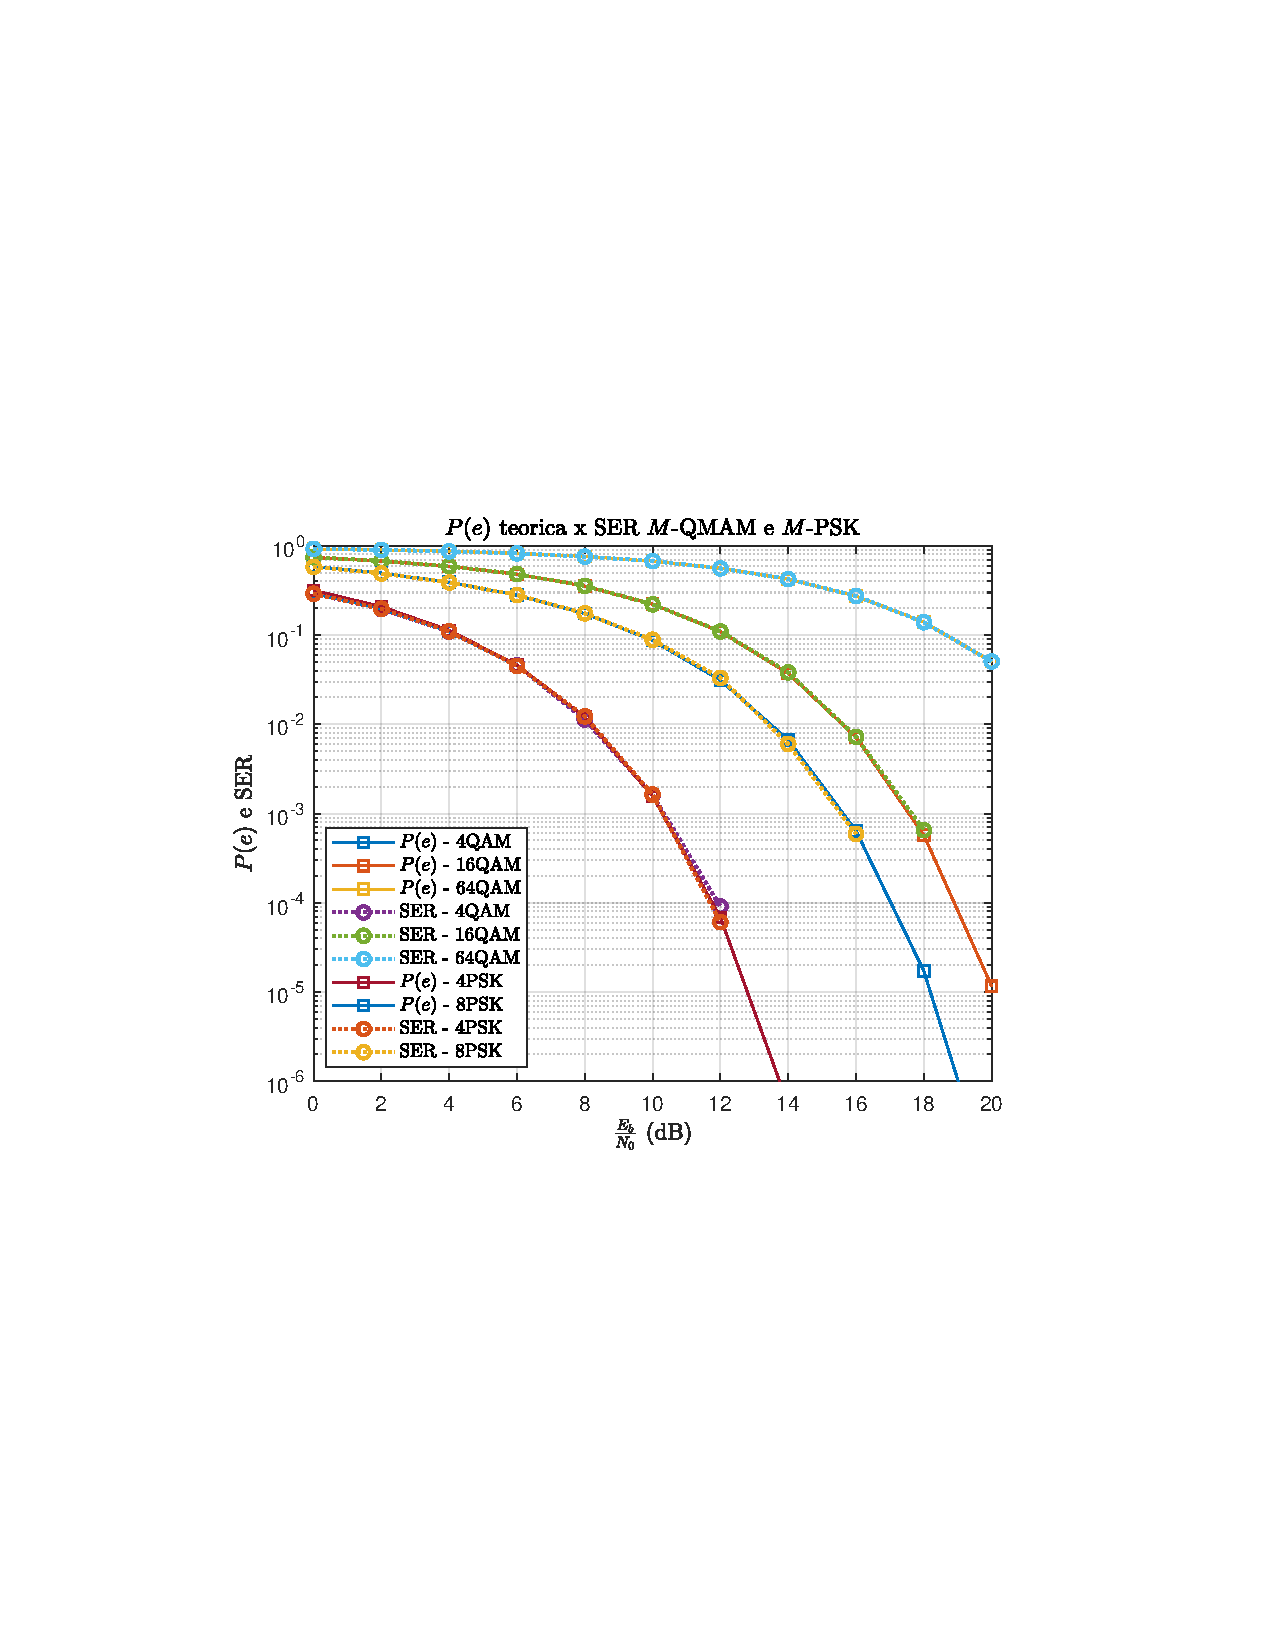
\includegraphics[width=1.0\textwidth,clip=true,trim={1.5cm 8.5cm 1.8cm 8.3cm}]{C:/Users/lukin/Documents/GitHub/Courses-HWs/Sistemas de Comunicacoes Digitais/matlab/problema5/fig/Erro_teoricaxAWGN_Geral.pdf}
    \caption{Probabilidade teórica de erro vs. simulação de transmissão $M$-PSK em canal RAGB.}
    \label{fig:Erro_teoricaxAWGN_Geral}
\end{figure}

\begin{figure}[!ht]
    \centering
    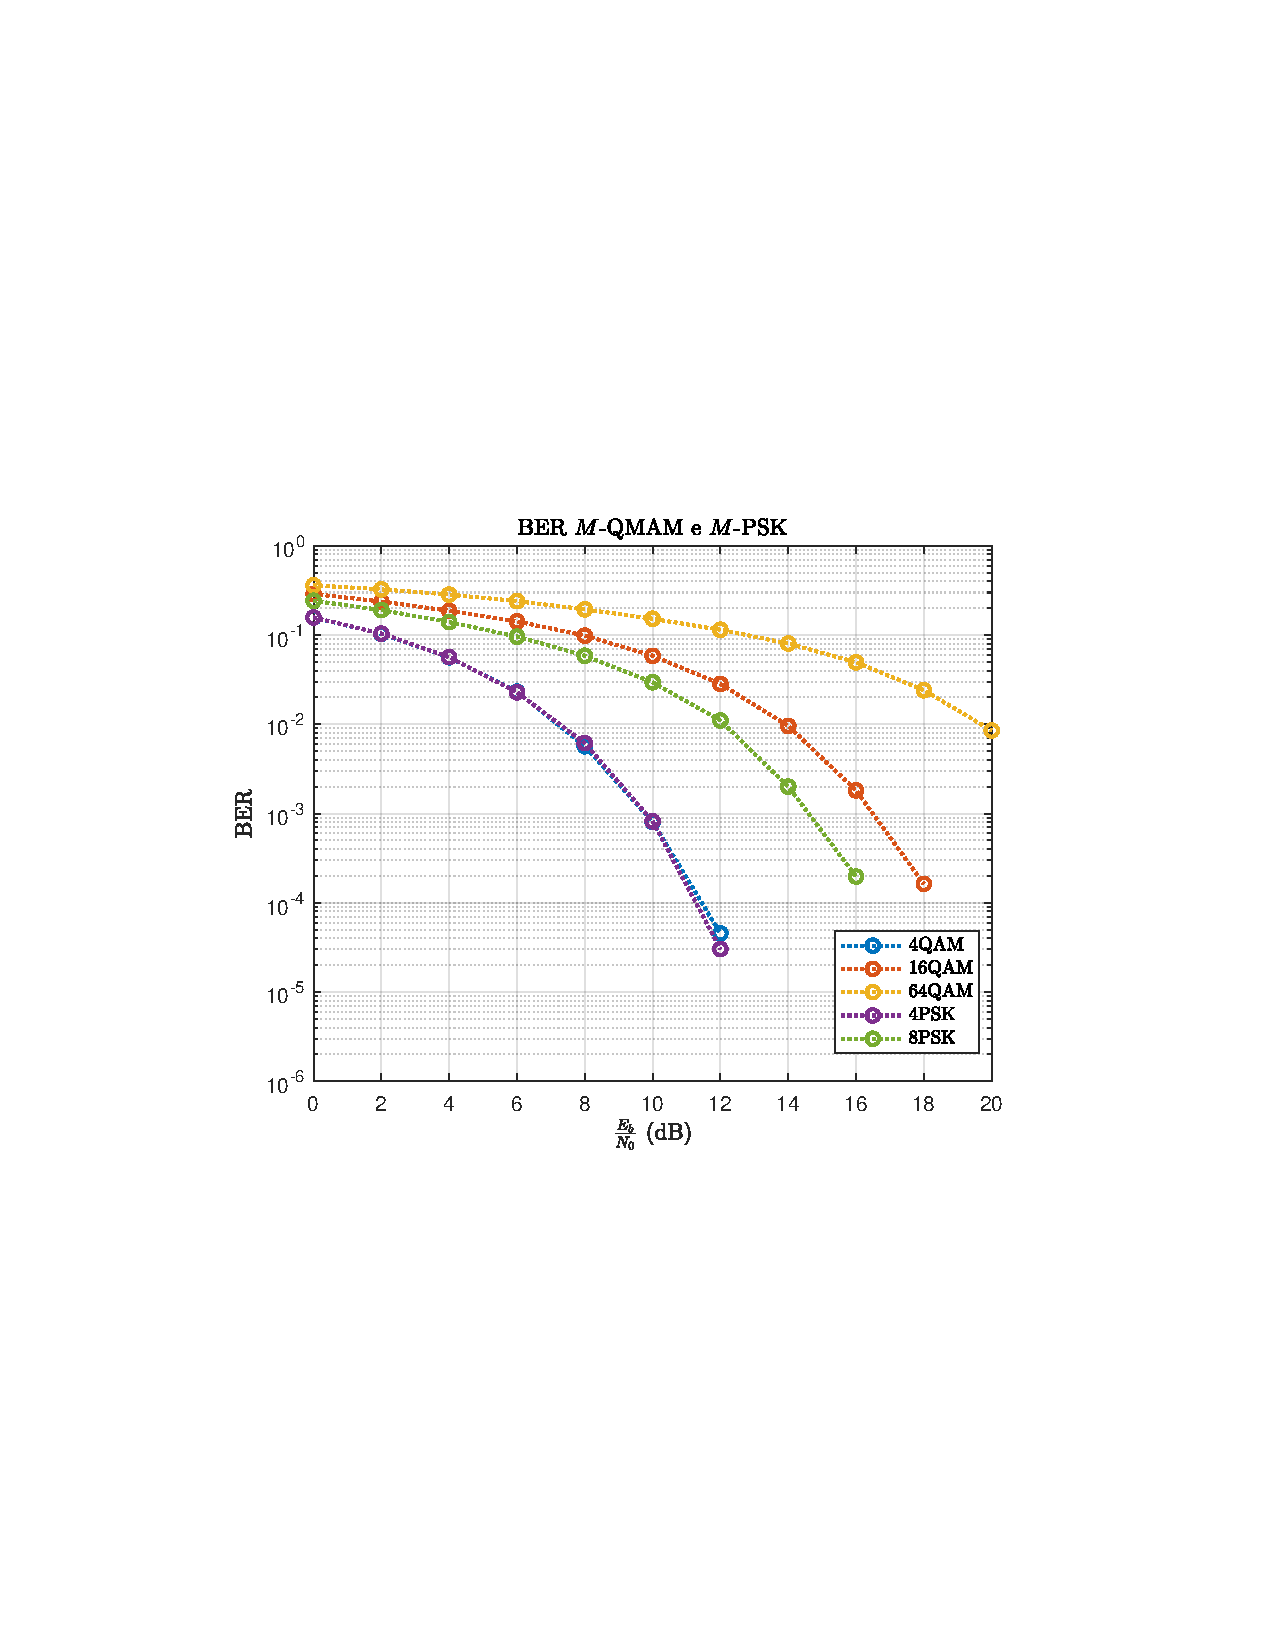
\includegraphics[width=1.0\textwidth,clip=true,trim={1.5cm 8.5cm 1.8cm 8.3cm}]{C:/Users/lukin/Documents/GitHub/Courses-HWs/Sistemas de Comunicacoes Digitais/matlab/problema5/fig/BER_teoricaxAWGN_Geral.pdf}
    \caption{Probabilidade teórica de erro vs. simulação de transmissão $M$-PSK em canal RAGB.}
    \label{fig:BER_teoricaxAWGN_Geral}
\end{figure}

